% Options for packages loaded elsewhere
\PassOptionsToPackage{unicode}{hyperref}
\PassOptionsToPackage{hyphens}{url}
%
\documentclass[
]{article}
\usepackage{lmodern}
\usepackage{amssymb,amsmath}
\usepackage{ifxetex,ifluatex}
\ifnum 0\ifxetex 1\fi\ifluatex 1\fi=0 % if pdftex
  \usepackage[T1]{fontenc}
  \usepackage[utf8]{inputenc}
  \usepackage{textcomp} % provide euro and other symbols
\else % if luatex or xetex
  \usepackage{unicode-math}
  \defaultfontfeatures{Scale=MatchLowercase}
  \defaultfontfeatures[\rmfamily]{Ligatures=TeX,Scale=1}
\fi
% Use upquote if available, for straight quotes in verbatim environments
\IfFileExists{upquote.sty}{\usepackage{upquote}}{}
\IfFileExists{microtype.sty}{% use microtype if available
  \usepackage[]{microtype}
  \UseMicrotypeSet[protrusion]{basicmath} % disable protrusion for tt fonts
}{}
\makeatletter
\@ifundefined{KOMAClassName}{% if non-KOMA class
  \IfFileExists{parskip.sty}{%
    \usepackage{parskip}
  }{% else
    \setlength{\parindent}{0pt}
    \setlength{\parskip}{6pt plus 2pt minus 1pt}}
}{% if KOMA class
  \KOMAoptions{parskip=half}}
\makeatother
\usepackage{xcolor}
\IfFileExists{xurl.sty}{\usepackage{xurl}}{} % add URL line breaks if available
\IfFileExists{bookmark.sty}{\usepackage{bookmark}}{\usepackage{hyperref}}
\hypersetup{
  pdftitle={Installing MATLAB and COMPECON Toolbox},
  pdfauthor={Matthew Aaron Looney},
  hidelinks,
  pdfcreator={LaTeX via pandoc}}
\urlstyle{same} % disable monospaced font for URLs
\usepackage[margin=1in]{geometry}
\usepackage{graphicx,grffile}
\makeatletter
\def\maxwidth{\ifdim\Gin@nat@width>\linewidth\linewidth\else\Gin@nat@width\fi}
\def\maxheight{\ifdim\Gin@nat@height>\textheight\textheight\else\Gin@nat@height\fi}
\makeatother
% Scale images if necessary, so that they will not overflow the page
% margins by default, and it is still possible to overwrite the defaults
% using explicit options in \includegraphics[width, height, ...]{}
\setkeys{Gin}{width=\maxwidth,height=\maxheight,keepaspectratio}
% Set default figure placement to htbp
\makeatletter
\def\fps@figure{htbp}
\makeatother
\setlength{\emergencystretch}{3em} % prevent overfull lines
\providecommand{\tightlist}{%
  \setlength{\itemsep}{0pt}\setlength{\parskip}{0pt}}
\setcounter{secnumdepth}{-\maxdimen} % remove section numbering

\title{Installing MATLAB and COMPECON Toolbox}
\author{Matthew Aaron Looney}
\date{8/23/2020}

\begin{document}
\maketitle

\hypertarget{software-and-computer}{%
\section{Software and Computer}\label{software-and-computer}}

In this course every student needs to have a laptop installed with a
computing software environment called MATLAB. You will also need the
add-on package called CompEcon Toolbox. Bring your laptop to each
lecture. This will allow you to work on programming drills in the class.
The following steps will explain how to install MATLAB on your laptop
and how to obtain and install the CompEcon Toolbox.

\begin{center}\rule{0.5\linewidth}{0.5pt}\end{center}

\hypertarget{installing-matlab-r2020a-on-mac-and-windows}{%
\subsubsection{Installing MATLAB R2020a on Mac and
Windows}\label{installing-matlab-r2020a-on-mac-and-windows}}

\begin{enumerate}
\def\labelenumi{\arabic{enumi}.}
\item
  Go to \url{https://www.mathworks.com/}
\item
  Login if you have a Mathworks account or click Create Account if you
  do not have one. \textbf{Note: use your TTU e-mail address.}

  \begin{itemize}
  \tightlist
  \item
    You can login by clicking the ``person'' icon in the upper right
    corner. If you do not have an account then click on the ``person''
    icon and create one.
  \end{itemize}
\item
  After you login to your account click on your name (or initals) in the
  upper right corner of the screen and select ``My Account''.
\item
  You will see a list of licenses. Select license 714225.
\item
  Click ``Download'' on the next page and ``R2020a'' on the subsequent
  page.
\item
  If prompted, select the appropriate operating system and the download
  will start.
\item
  Run the installer from the downloaded file and follow the instructions
  to install MATLAB. This might take some time so plan accordingly to
  allow the install/download to complete without interruption.
\item
  MATLAB is now installed.
\end{enumerate}

\hypertarget{installing-compecon-toolbox-on-mac-and-windows}{%
\subsubsection{Installing CompEcon Toolbox on Mac and
Windows}\label{installing-compecon-toolbox-on-mac-and-windows}}

Many of the examples we study in this class will be taken from Miranda
and Fackler's book, Applied Computational Economics and Finance. The
model solvers developed by the authors and the MATLAB scripts for
solving the examples in the book can be downloaded as a package called
``CompEcon Toolbox'' from the authors' website
\url{https://pfackler.wordpress.ncsu.edu/compecon/}.

\begin{enumerate}
\def\labelenumi{\arabic{enumi}.}
\item
  Download CompEcon Toolbox from
  \url{https://pfackler.wordpress.ncsu.edu/compecon/154-2/}
\item
  I suggest you install the 64-bit version of the software.
\item
  After the file downloads, locate the file on your computer. It will be
  called ``compecon2011\_64\_20110718.zip'' if you downloaded the 64-bit
  version.
\item
  When you installed MATLAB a directory was created in your
  ``Documents'' folder called ``MATLAB''. I suggest you copy the
  downloaded file ``compecon2011\_64\_20110718.zip'' into your MATLAB
  folder.
\item
  Unzip the file called ``compecon2011\_64\_20110718.zip''. This will
  create a folder called ``compecon2011\_64\_20110718''.
\item
  At this time I suggest you create a second folder in your MATLAB
  folder called ``Optim\_Class\_Fall\_2020''. This is optional but
  useful. You can place all materials from the class in this folder.
\item
  CompEcon Toolbox is now installed.
\end{enumerate}

\hypertarget{setting-the-path-in-matlab-on-mac-and-windows}{%
\subsubsection{Setting the Path in MATLAB on Mac and
Windows}\label{setting-the-path-in-matlab-on-mac-and-windows}}

For MATLAB to find the files (CompEcon Toolbox and script files) on your
computer you need to tell MATLAB where the files are located. The
easiest way to do this is to ``Set Path'' to your MATLAB folder inside
your Documents folder.

\begin{enumerate}
\def\labelenumi{\arabic{enumi}.}
\item
  Open the MATLAB program.
\item
  Click on the ``HOME'' tab in the upper left corner.
\item
  You will see a button called ``Set Path''. Click the button.
\item
  You will see a screen that looks like the following:
\end{enumerate}

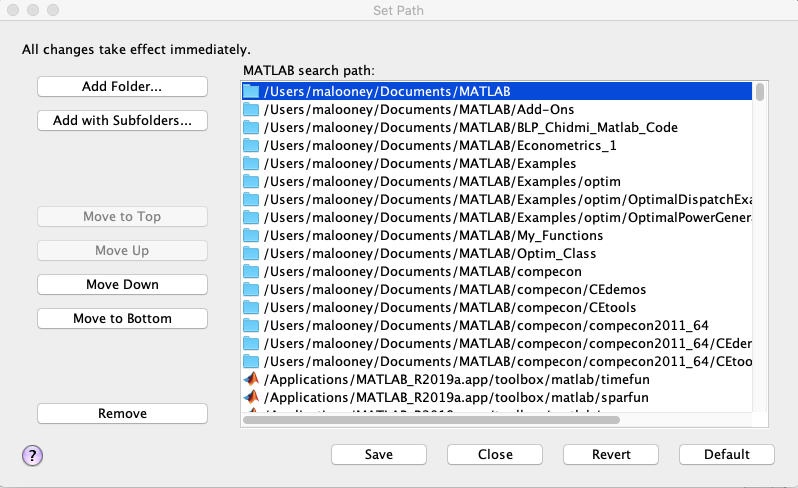
\includegraphics[width=0.75\textwidth,height=\textheight]{/Users/malooney/Documents/malooney.github.io/Optim_Class_Fall2020/softwareInstall/setPath.png}

\begin{enumerate}
\def\labelenumi{\arabic{enumi}.}
\setcounter{enumi}{4}
\item
  Click on the ``Add with Subfolders\ldots{}'' button.
\item
  Navigate to your Documents folder and select the MATLAB folder. Click
  ``Open'' (on Mac) or ``Select Folder'' (on Windows).
\item
  Click ``Save'' and then ``Close''.
\item
  The path is now set. Anything saved inside your MATLAB folder will now
  be visible to MATLAB.
\item
  If you created a folder called ``Optim\_Class\_Fall\_2020'' in your
  MATLAB folder then all you need to do is simply copy files into this
  folder and the files will be automatically added to the MATLAB path.
  EASY!
\end{enumerate}

\hypertarget{compiling-the-compecon-toolbox}{%
\subsubsection{Compiling the CompEcon
Toolbox}\label{compiling-the-compecon-toolbox}}

For the CompEcon Toolbox to function properly we need to compile some
code. If you have never compiled code before this can sound scary but I
assure you the process is not very complicated.

\hypertarget{for-mac-users}{%
\paragraph{For Mac users}\label{for-mac-users}}

We need to install the ``Xcode command line tools''.

\begin{enumerate}
\def\labelenumi{\arabic{enumi}.}
\item
  Open the ``Terminal'' application. This is inside the ``Utilities''
  folder inside the main ``Applications'' folder on your hard drive.
\item
  At the command prompt, type ``Xcode-select --install''.
\item
  Once the install is complete open the MATLAB application.
\item
  In the ``Command Window'' type, ``mexall''.
\item
  The CompEcon Toolbox code will start to compile. Wait until it is
  done.
\item
  Your code is now compiled\ldots EASY!!
\end{enumerate}

\hypertarget{for-windows-users}{%
\paragraph{For Windows users}\label{for-windows-users}}

We need to download a Windows compatible compiler. The easiest compiler
to use is ``Mingw-w64 - GCC for Windows 64 \& 32 bits''.

\begin{enumerate}
\def\labelenumi{\arabic{enumi}.}
\item
  Open the MATLAB application and click on the ``HOME'' tab.
\item
  Click on the ``Add-Ons'' button in the upper right of the screen.
\item
  The ``Add-On Explorer'' will open.
\item
  In the upper right of the screen there is a search bar. Type
  ``MinGW-w64'' and hit enter.
\item
  The following screen will appear:
\end{enumerate}

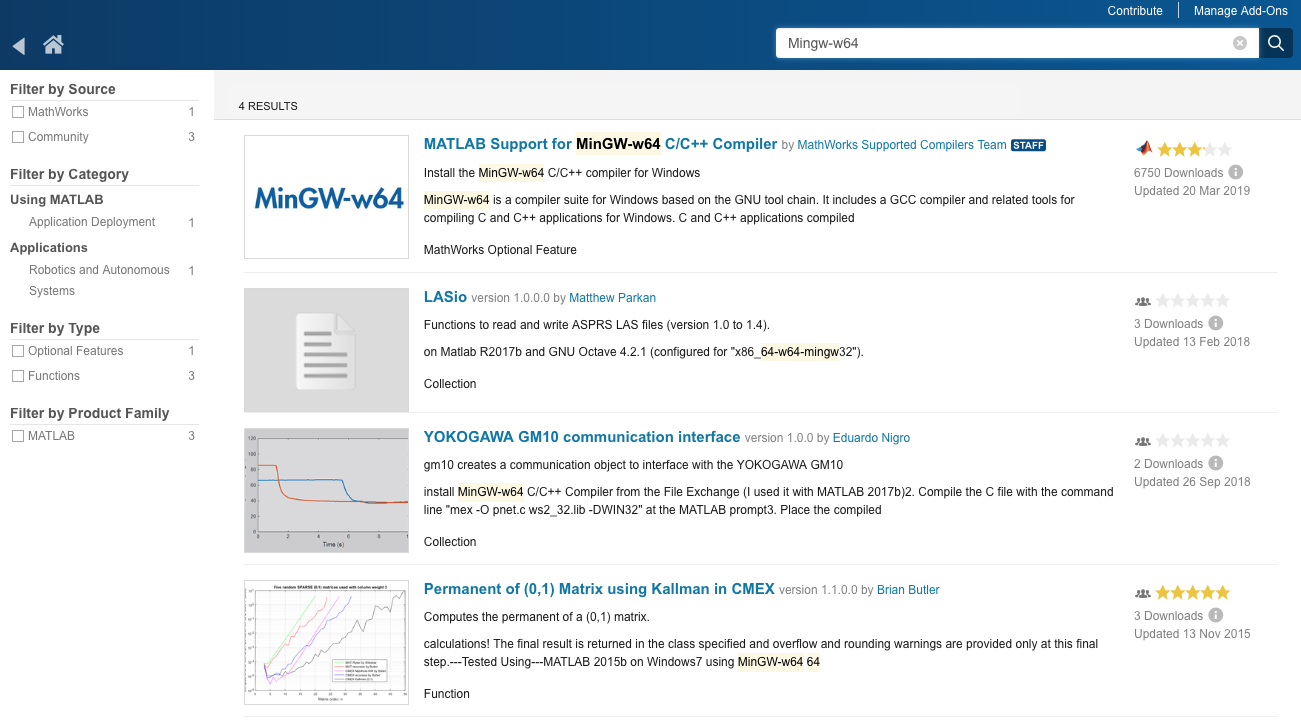
\includegraphics[width=0.75\textwidth,height=\textheight]{/Users/malooney/Documents/malooney.github.io/Optim_Class_Fall2020/softwareInstall/Mingw.png}

\begin{enumerate}
\def\labelenumi{\arabic{enumi}.}
\setcounter{enumi}{5}
\item
  Click on ``MATLAB Support for MinGW-w64 C/C++ Compiler'' and click the
  ``Install'' button. Follow the directions for installing the compiler.
\item
  Once the install is complete, close the ``Add-On Explorer''.
\item
  In the ``Command Window'' of MATLAB, type, ``mexall''.
\item
  The CompEcon Toolbox code will start to compile. Wait until it is
  done.
\item
  Your code is now compiled\ldots EASY!!
\end{enumerate}

\hypertarget{renaming-the-psi-function-in-compecon-toolbox}{%
\subsubsection{Renaming the ``Psi'' function in CompEcon
Toolbox}\label{renaming-the-psi-function-in-compecon-toolbox}}

We are almost done.

There is one small issue with the CompEcon Toolbox. MATLAB has a
built-in function called ``Psi.c''. However, CompEcon Toolbox also has a
function called ``Psi.c''. This throws a warning message when you start
MATLAB after installing and compiling CompEcon Toolbox.. The easy
workaround solution is to rename the CompEcon Toolbox function ``Psi.c''
to something else.

None of the scripts we will use in this class require use of the Psi.c
function but you need to keep in mind that we are renaming the ``Psi.c''
function so if in the future you use a script that requires use of the
``Psi.c'' function from CompEcon Toolbox you will need to rename that
inside the script file also. This sounds convoluted and complicated but
it is not. It is just hard to explain in words. The action is very
simple.

\begin{enumerate}
\def\labelenumi{\arabic{enumi}.}
\item
  Open the MATLAB folder inside your Documents folder.
\item
  Open the CompEcon folder.
\item
  Open the CEtools folder and scroll down until you find the file named
  ``Psi.c''.
\item
  I suggest you rename all ``Psi.x'' files to ``Psi\_cet.x'', where
  ``x'' represents the file extension and ``cet'' stands for compecon
  toolbox. For example, the file called ``Psi.c'' will be renamed to
  ``Psi\_cet.c''. Depending on the version of CompEcon Toolbox you
  installed you should have about six files to rename. Rename them all.
\item
  Once you have done this restart MATLAB. You should not see any warning
  notices about the Psi function. If you do you have missed renaming a
  file.
\end{enumerate}

\begin{center}\rule{0.5\linewidth}{0.5pt}\end{center}

\hypertarget{you-should-now-have-a-fully-functioning-version-of-matlab-installed.}{%
\subsubsection{You should now have a fully functioning version of MATLAB
installed.}\label{you-should-now-have-a-fully-functioning-version-of-matlab-installed.}}

\hypertarget{you-should-now-have-the-compecon-toolbox-installed.}{%
\subsubsection{You should now have the CompEcon Toolbox
installed.}\label{you-should-now-have-the-compecon-toolbox-installed.}}

\hypertarget{your-path-should-be-set-to-the-matlab-folder-inside-your-documents-folder.}{%
\subsubsection{Your Path should be set to the MATLAB folder inside your
Documents
folder.}\label{your-path-should-be-set-to-the-matlab-folder-inside-your-documents-folder.}}

\hypertarget{you-should-have-all-code-compiled.}{%
\subsubsection{You should have all code
compiled.}\label{you-should-have-all-code-compiled.}}

\hypertarget{you-should-not-see-any-warning-notices-when-starting-matlab.}{%
\subsubsection{You should not see any warning notices when starting
MATLAB.}\label{you-should-not-see-any-warning-notices-when-starting-matlab.}}

\bigskip
\bigskip

\centering

\hypertarget{if-you-had-trouble-with-any-of-these-steps-please-get-in-touch-with-me-and-i-can-help-guide-you-through-the-process.}{%
\section{If you had trouble with any of these steps please get in touch
with me and I can help guide you through the
process.}\label{if-you-had-trouble-with-any-of-these-steps-please-get-in-touch-with-me-and-i-can-help-guide-you-through-the-process.}}

\end{document}
